\section{Concept}
\subsection{Basic Concept}
Feet are used in many real world tasks together with the rest of the body, but in computer environments they are almost completely put aside as an interaction possibility \cite{pakkanen}. For instance, Ubicomp researches have develop different types of interfaces for public spaces where users' hands are the protagonists and feet are partly or completely neglected. 

The basic concept of this project is a feet-based interface whose \textbf{individual modules} react when pushed or kicked. For this purpose, modules have to be highly \textbf {mobile} to yield a flexible interaction with the user. Another desired aspect is \textbf {expandability}: the envisioned system will allow the integration of new modules and features. %search literature to support this 
Finally, a module is expected to detect if a another module comes up against it. In other words, another feature in the envisioned system is the \textbf{interaction between modules}. 

%So a server - client - structure is a very broad system and maybe to powerful for the target of this project. 
%First idea was to build several independent hardware devices which communicate between each other. But the usage of a server - client based system has plenty more advantages than to build a simple hardware - communication - system:
%Furthermore an administrator can change the device defaults pretty easy using the Graphical Interface.   

\subsection{Hardware Concept}
To achieve \textbf{modularity} and \textbf{mobility}, a wireless communication platform is fundamental.   
Panstamps, as explained in [{\url{http://www.panstamp.com/home}}], are small boards intended for implementing custom wireless networks. In their boards, Panstamps have an integrated transceiver, the CC1101, that makes the wireless communication possible. %add reference to CC1101

Due to Panstamps' open source nature, documentation and information about already implemented projects with them is at hand for everyone on the internet; this represents a very important advantage over other wireless products in the market. %search source that supports this 
Furthermore, Panstamps' core is the the ATMEGA 328 [{\url{http://www.atmel.com/devices/atmega328.aspx}}]; therefore, they are entirely programmable from the Arduino IDE, whose community is increasing each day.%search literature to support this

For all these reasons, we decided to build the envisioned system upon Panstamps. As depicted in Figure~\ref{fig:server-module}, each module in our system is constituted by a sensor and actuator node, both having a Panstamp as their nucleus. The server node has also a Panstamp as its main component, which communicates wirelessly with the other modules' panstamps. 

The Java Server gets the data recollected by the server node, process it and gives a response to the server node that has to be sent to the appropriate node in the network. The feedback provided by the Java Server depends entirely on the \emph{personality} of each device. For a better understanding of \emph{Personalities}, please refer to the XXX section of this work.

\begin{figure}[h!]
 \centering
 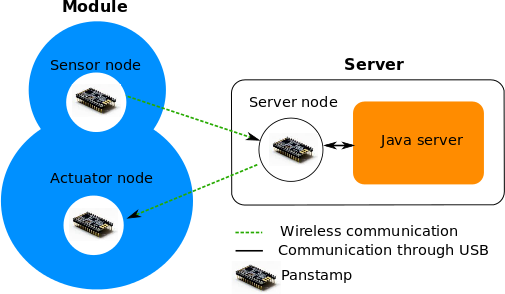
\includegraphics[width= 0.4\textwidth, clip=true  ,keepaspectratio=true]{./graph/entity_server.png}
 \caption{Interface's server and a module}
 \label{fig:server-module}
\end{figure}

To detect if they have been kicked or pushed, modules need to sense their own movement; therefore, an accelerometer is connected to the sensor node of each module as shown by Figure \ref{fig:sensor-node}. We used the ADXL335, a small accelerometer that measures acceleration in each of the cardinal directions (x,y and z).

Each module has a led strand constituted by led-and-controller pairs. To produce a certain light pattern, the actuator node, which is connected to the strand (see Figure \ref{fig:actuator-node}), sends information to each controller to indicate whether its led should be on or off and what color has to be displayed. Led patterns play an important role in the interface because each module expresses its \textbf{personality} through led patterns.  

The \textbf{interaction between modules} is based on contact; that is, a module triggers a reaction in other module only when it touches it. In our implementation, the closeness between two modules is determined by measuring the RSSI of broadcasted messages in the network. As explained in (add reference here!), the RSSI is a measurement of the power present in a received radio signal. The longer the distance travelled by a radio wave the bigger its intensity loss; hence,    


All the elements in a module are powered by a 11 volts Li-Po battery. This battery should not be over-discharged, for this reduces drastically it's life. Therefore, sensor nodes have an integrated voltage-monitoring circuit (see Figure \ref{fig:sensor-node}) with which the low-battery state is detected.

\begin{figure}[h!]
 \centering
 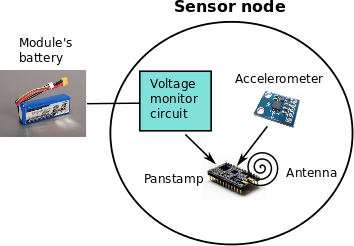
\includegraphics[width= 0.4\textwidth, clip=true  ,keepaspectratio=true]{./graph/sensor_node.png}
 \caption{Sensor node elements}
 \label{fig:sensor-node}
\end{figure}


\begin{figure}[h!]
 \centering
 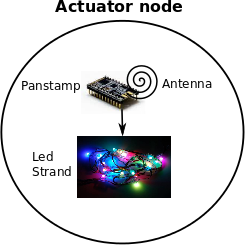
\includegraphics[width= 0.3\textwidth, clip=true  ,keepaspectratio=true]{./graph/actuator_node.png}
 \caption{Actuator node elements}
 \label{fig:actuator-node}
\end{figure}


%schematic of the battery monitor circuit
%overall schematic of a sensor node
%schematic of a actuator node
%packets structure

\subsection{Software Concept} 

\subsubsection{Driver} 
Since we used the Arduino IDE to program the Panstamps, all the nodes' drivers in the network were written in C++. The driver was designed to allow \textbf{expandability}; as a result, new nodes can be added to the network by coping the basic drivers and changing them slightly. 

In short, the driver is in charge of:
\begin{itemize}
\item enabling the wireless communication
\item managing the communication between different nodes
\item handling the information provided by sensors 
\item operating the led strands
\item setting up the communication with the Java Server on the Panstamp' side
\end{itemize}

\subsubsection{Java server}

The Java Server is the heart of the interface; in other words, it is the orchestrator of all nodes in the system's network. The server node transfers all the data gathered in the network to the Java Server, which produces a response according to each module's personality and sends it to the intended actuator nodes through the server node (See ~\ref{fig:server-module}).  


It is also possible to put the server software on a more powerful microcontroller like a raspberry pi or some similar controller.
The modularity is given through a number of easy configurable files. Changing behavior, appearance or the defined actions is pretty easy to do.

The system contains the different hardware devices and the server. The communication is enabled by using panstamps. When one of the devices gets activated by e.g. kicking it, the accelerometer sensor will trigger an input sending it to the panstamp. There a packet will be created which contains the ID of the device, the intensity of the kinetic input and a checksum bit at the end.
The kinetic inputs "first contact", "played" and "played hard" are triggered by each other:
So when the device gets kicked, his state will change from "standby" to "first contact", then when the threshold is high enough, the state changes directly to "played". There cannot be a change from "first contact" to "played hard". 
% !!weitere daten des paketes
Those data will be send to the panstamp of the server where this data will be analyzed and compared to the corresponding personality of the device. The personality then outputs the behaviour for the device. A behaviour consists two colors (which can be the same) and a pattern. This pattern describes the appearance of the colors. (Like a blinking or fading of the LEDs)
The idea was to create typical characters for the devices. Below you can see the table which describes how a device reacts to kinetic inputs into his environment. So if it is in his default state the device "Paul" is fading blue. By changing input the state will change perhaps to the state "hard played". Those behaviour can be manipulated using the servers graphical interface. The % INSERT DEVICE - STATE TABLE
The next table indicates the behaviour of the personalities to each other. Using the antennas field  it is possible to identify directly neighboured devices. But the usage of this effect is really not exact, because the antennas must be parallel to each other. So apparently most time when two devices got in contact there won't be a "found neighbour" - message. The devices have to be both in right position. This means that the antennas have to be rightly erected. (The ground has to be on bottom side.)   
So by using this technique the following rules shown in this table can be implemented.
When the servers got from the device panstamp the data with which other device it is confronted, the server looks up in the data of the presetpersonalities.java file and returns the matching pattern. For this use it is necessary to define which personality is more dominant than another.
The table below shows how the different personalities will interact to each other.
% INSERT DEVICE -DEVICE TABLE
For sure there is no interaction when "Paul" gets in touch with another "Paul" (because there should only be one Paul) but by using the servers settings it is quite easy to do so. There won't be any interaction between the same personalities.

So when the server has received the data of its state and his neighbourhood of the sending device it will send a new pattern for the LEDs chain actuator when the situation of the sending device has changed.
When the device hadn't send its data packet for two minutes a warning will pop up in the graphical interface. Apparently this will happen when the device is out of range of the sending area of the panstamp antennas (approximately ~50 metres).
This very functionality is illustrated in the following graphic.
% INSERT GRAPHICAL PICTURE OF FUNCTIONALITY OF THE SERVER-CLIENT-SYSTEM       
 
% used technologies
One of the projects constrains in the beginning was to build something based on the Arduino technology, because there is a lot of open - source code in the internet and it is easy to learn.
Another constraint was to write the servers code in Java. Because the servers environment of this project should be similar to other ancient projects at this chair.
Later, when the work began it was necessary to find a hardware module for the devices which is sending and receiving the data packages to and from the server. Some experiments with XBees indicated that the commuting area is pretty to small to have a good functionality of the system. (In fact the server lost signal already when the Device was just approximately five metres apart.) So the work with the panstamp began.   
 

